\documentclass[12pt,titlepage]{article}
\usepackage[spanish]{babel}
\usepackage[utf8]{inputenc}
\usepackage{amsfonts}
\usepackage{amsmath}
\usepackage{amssymb}
\usepackage{color}
\usepackage{graphicx} % para insertar imagenes
\usepackage{caratulaMetNum}
\usepackage{verbatim}
\usepackage{float}


\newcommand{\func}[2]{\texttt{#1}(#2)}
\newcommand{\funcFull}[2]{\texttt{#1}=#2}
\newcommand{\tab}{\hspace*{2em}}
\newcommand{\FOR}{\textbf{for }}
\newcommand{\END}{\textbf{end }}
\newcommand{\TO}{\textbf{ to }}
\newcommand{\IF}{\textbf{if }}
\newcommand{\WHILE}{\textbf{while }}
\newcommand{\THEN}{\textbf{then }}
\newcommand{\ELSE}{\textbf{else }}
\newcommand{\RET}{\textbf{return }}
\newcommand{\MOD}{\textbf{ \% }}
\newcommand{\OR}{\textbf{ or }}
\newcommand{\AND}{\textbf{ and }}
\newcommand{\tOde}[1]{\tab \small{O($#1$)}}
\newcommand{\Ode}[1]{O($#1$)}
\newcommand{\Thetade}[1]{{\small$\Theta$($#1$)}}
\newcommand{\Omegade}[1]{{\small$\Omega$($#1$)}}
\newcommand{\VSP}{\vspace*{3em}}
\newcommand{\pa}{\vspace{5mm}}
\newcommand{\e}[2]{\varepsilon  _{#1}({#2})}
\newcommand{\er}[2]{\varepsilon _{({#1})}^{({#2})}}
\newcommand{\ev}[1]{\varepsilon _{#1}}
\newcommand{\N}{\mathbb{N}}
\newenvironment{pseudo}{\begin{tabular}{p{11cm}l}}{\end{tabular}\VSP}


\newcommand{\gra}[1]{{\noindent\centering\includegraphics[width=14cm]{#1}}\\}

\begin{document}

\materia{Métodos Numéricos}
\titulo{Trabajo Práctico Nº3}
\subtitulo{Más que Splines}
\integrante{Carla Livorno}{424/08}{carlalivorno@hotmail.com}
\integrante{Mariano De Sousa Bispo}{389/08}{marian\_sabianaa@hotmail.com}

\abstracto{
	El siguiente trabajo se propone la implementación de una curva paramétrica mediantes $splines$ naturales a partir de un conjunto de puntos.\\
	Además, la curva provee la funcionalidad de seleccionar un punto cualquiera de la misma (generalmente este punto se encuentra meramente $cerca$ de la curva) y moverlo a una nueva posición modificando la curva.
}

\palabraClave{Spline cúbico natural}
\palabraClave{Curva paramétrica}
\palabraClave{Polinomios}

\begin{titlepage}
\maketitle
\end{titlepage}
\tableofcontents
\newpage
	\begin{section}{Introducción teórica}	
	Multitud de problemas de la vida real se rigen por proporciones constantes entre las magnitudes implicadas: procesos físicos, reacciones químicas, costes de materias primas y sus relaciones para formar otros producto, etc.
	Todas estas situaciones admiten de forma natural una descripción matemática a través de sistemas de ecuaciones lineales.
	Además estos sistemas son útiles como una buena aproximación a sistemas más complejos o sistemas de ecuaciones no-lineales.
	
	La resolución de muchos problemas conlleva el manejo de gigantescos sistemas de ecuaciones lineales, por lo que es necesario plantearse métodos eficientes para su análisis.
	
	Los sistemas de ecuaciones lineales son un conjunto de $m$ ecuaciones relacionadas en $n$ variables. Se los puede expresar en forma matricial como $A \dot x = b$ donde $A$ es una matriz de $m \times n$, $x$ es un vector columna de tamaño $n$ y $b$ un vector de tamaño $m$.
	
	Existen diversos métodos para la resolución de estos sistemas de ecuaciones. Haremos una breve introducción a los distintos métodos.
	
	Tenemos por un lado los métodos iterativos como es el caso del método de Jacobi, Gauss-Seidel o del Gradiente Conjugado que como su nombre lo indica se los aplica en forma iterativa para lograr una aproximación a la solución real del sistema en cuestión
	
	Por otra parte, existen los denominados métodos directos entre los cuales se encuentra el método de eliminación de Gauss el cual es una forma directa para llegar en un número finito de pasos a un sistema equivalente pero mas simple, la factorización LU que se vale de este último, la descomposición de Cholesky, y la descomposición QR.
\end{section}

	\newpage
	\begin{section}{Desarrollo}
	\begin{subsection}{Explicación}
		\begin{subsubsection}{Introducción al problema}
			La guerra lineal consiste en dos naves situadas en el hiperespacio de $n$ dimensiones con el objetivo de desintegrarse mutuamente mediante disparos de cañones $Warp$.\\
			
			Cada turno del combate consiste en lo siguiente:
			\begin{enumerate}
			\item Nos proveen la matriz $A'$ usada por el oponente para atacarnos y el punto $d'$ donde impactó el proyectil. Con esa información debemos intentar descubrir la posición $y$ donde se encuentra situada la nave enemiga, es decir, resolver el sistema $A'y=d'$.
					
			\item Tenemos la posición a la que pretendemos disparar ($d$) y queremos conseguir una matriz de ataque $A$ tal que $Ax=d$ donde $x$ es nuestra posición.
			\end{enumerate}
		\end{subsubsection}
		\begin{subsubsection}{Estrategia}
			En cada turno nuestra estrategia consiste en lo siguiente:
			
			\begin{enumerate}
			\item Para resolver el sistema $A'y=d'$ decicimos usar métodos directos de resolución de sistemas de ecuaciones lineales. La elección se basa en que los métodos iterativos calculan $aproximaciones$ a la solución por lo que los elegiríamos sólo en el caso de no conocer un método que calcule la solución de forma $exacta$ o que este, sea muy costoso.
				\begin{itemize}
					\item \underline{Opción 1:} Buscamos la matriz inversa de A' (existe porque es parte de las reglas de la batalla) mediante el método de eliminación Gaussiana. Es decir, efectuamos a la matriz A' distintas trasformaciones lineales hasta convertirla en la matriz identidad. Al mismo tiempo hacemos dichas trasformaciones a la matriz identidad quedando en esta la inversa de A'.
					Las transformaciones consisten en triangular superior e inferiormente A' y poner $unos$ en la diagonal.
					Una vez que conocemos la inversa ($A'^{-1}$) podemos hallar la posición buscada de la siguiente manera: $y=A'^{-1}*d'$.\\
					
					\item \underline{Opción 2:} Hallamos la factorización $LU$ de $A'$ (si no existe, conseguimos $PLU$). Resolvemos el sistema $LUy=d'$. LLamamos $Ux=z$ y resolvemos usando sustitución hacia adelante el sistema $Lz=d'$. Una vez que conocemos $z$ obtenemos $x$ tal que $Ux=z$ utilizando sustitución en reversa. (Con $PLU$ es el mismo procedimiento pero permutando $d'$ según $P$).\\
					
					Elegimos este método ya que las matrices son cuadradas. Además, la implementación es sencilla y la complejidad algorítmica del método es razonable ya que se trata de un algoritmo de orden cúbico.
				\end{itemize}
			
				La exactitud con la que calculemos la posición buscada $y$ depende del número de condición de la matriz $A'$, cuanto mayor es este número menor es la precisión del resultado obtenido. Se considera que alcanzamos al rival cuando $\left|| y' - y \right|| \leq 1$, donde $y'$ es la solución encontrada.
				
				Como creemos que el adversario va a utilizar matrices mal condicionadas para atacarnos, en cada turno estaríamos calculando una posición errada de donde se encuentra. Por este motivo, decidimos usar la estrategia de disparar en el punto promedio de todas las posiciones calculadas hasta el momento del ataque (utilizando la información de los ataques previos). Esperamos de esta manera ir obteniendo cada vez mejores aproximaciones a donde se encuentra realmente.
			
			
			\item Para atacar necesitamos una matriz $A$ que al multiplicarla por nuestra posición resulte en un impacto en la posición deseada $d$. Es decir, necesitamos que $A$ cumpla $Ax=d$.
			
			Sea $n$ la dimensión de $A$.
			Dado que tenemos $n^2$ incognitas y $n$ ecuaciones, tenemos $n^2-n$ elementos de $A$ libres. Por este motivo, podemos elegir $A$ convenientemente y luego adaptarla (forzarla a cumplir $Ax=d$).			
			
			Como debemos proveer al adversario de la matriz $A$ que usemos para el ataque tenemos que idear una estrategia para que nuestra posición no sea descubierta en el siguiente turno. La estrategia consiste en generar matrices mal condicionadas que a su vez sean inversibles (esto último por reglamento). En algunos turno usamos la matriz de Hilbert multiplicada por un escalar. 
			
			Para crear una matriz mal condicionada, generamos un único vector aleatorio de dimensión $n$ que resulta en las filas de dicha matriz. De esta manera tenemos una matriz cuyas filas son linealmente dependientes, por lo que la matriz no es inversible. Luego, sumamos a los elementos de la diagonal un $epsilon$ (Ver en las pruebas (secciones \texttt{Resultados} y \texttt{Discusión}) como fue elegido) obteniendo asi una matriz inversible y mal condicionada. En este tipo de matrices el determinante tiende a $cero$, es decir, a pesar de ser inversible, esta muy cercana a dejar de serlo.
			
			Por último, para forzarla a satisfacer el sistema elegimos una columna $j$ de $A$ tal que el $j-esimo$ elemento de $x$ sea distinto de $cero$ ($x$ no es el vector nulo por precondición ya que es nuestra posición), sino los coeficientes de $A$ que pretendemos setear no tienen importancia, y consideramos incognitas sólo a los coeficientes de esa columna. Nos quedan así, $n$ incognitas y $n$ ecuaciones, por lo que podemos despejarlas y obtener la matriz final.
			
			La matriz obtenida sigue siendo inversible ya que modficamos sólo una columna de la misma y lo que hace linealmente independiente a las filas son los elementos de la diagonal.
			
			\underline{Nota:} Al momento de obtener la matriz de ataque, pedimos un número random entre el 0 y el 9, si obtenemos el 0 usamos un múltiplo de la matriz de Hilbert, sino generamos una matriz mal condicionada como explicamos previamente.
			\end{enumerate}
		\end{subsubsection}
	\end{subsection}
	\begin{subsection}{Implementación}
		En primer lugar el desarrollo consistió en implementar módulos para las operaciones entre Matrices y Vectores que fueran necesarias para resolver sistemas lineales. Esto implicaba también implementar el algoritmo de factorización LU y el algoritmo de eliminación Gaussiana ambos con pivoteo parcial para resolver el sistema lineal.\\
		
		Escribimos el módulo \texttt{Matrix} que implementa una matriz en $\mathbb{R}^{nxn}$ con las siguientes operaciones:\\
		
		\begin{tabular}{rl}
			\texttt{Eliminación Gaussiana} & Eliminacion Gaussiana con pivoteo parcial.\\
			\texttt{LU} & Factorización LU con pivoteo parcial.\\
			\texttt{Inversa} & Matriz inversa con el método de Gauss.\\
			\texttt{K} & Número de condición.\\
			\multicolumn{2}{l}{
				\texttt{Suma, Resta, Multiplicación, Multiplicación por escalar, traspuesta}
			}
		\end{tabular}\\
		
		Usamos pivoteo parcial tanto para la eliminación Gaussiana como para la factorización LU para reducir el error de redondeo en las operaciones.\\
		
		Además escribimos la clase \texttt{Vector} que implementa un vector en $\mathbb{R}^n$ con las operaciones básicas como \texttt{Suma, Resta,
		Producto Escalar, Producto Vectorial, Normas}, etc.\\
		
		\underline{NOTA:} Ambas clases heredan de una clase \texttt{MatrixBase} que implementa las funciones básicas como son la suma, resta, multiplicación, etc.\\
		
		Teniendo la base (matrices, vectores y las operaciones entre ellos) implementamos una clase para la resolución de sistemas de ecuciones lineales y una clase para elegir la matriz de ataque.\\
		
		El módulo \texttt{linearSystem} implementa las siguientes funciones:\\
		
		\begin{tabular}{rl}
			\texttt{Resolución por inversa} & consigue la inversa y hace la multiplicación.\\
			\texttt{Resolución por LU} & consigue LU (PLU) y despeja el sistema usando\\
									   & sustitución hacia adelante y sustitución reversa.\\
		\end{tabular}\\
		
		El módulo \texttt{warpCannon} implementa las siguientes funciones:\\
		
		\begin{tabular}{rl}
			\texttt{Atacar} & consigue la posición de impacto deseada y arma la matriz correspondiente.\\
		\end{tabular}\\
		
		Esta clase tiene un método privado que calcula la posición del enemigo.
		
		Nuestra primer idea fue hacer un promedio coordenada a coordenada dandole una distinta prioridad a cada vector (posición), dicha prioridad dependía del número de condición de la matriz que uso el oponente en ese turno. Es decir, $y$ tiene mayor prioridad que $z$ si y sólo si $K(A')<K(A)$ siendo $A'y=d'$ y $Az=d$.
		
		Para lograr esto, teníamos un $array$ de $tuplas$ donde la primer coordenada correspondía al vector y la segunda al número de condición de la matriz asociada.
		
		La idea finalmente implementada es una versión más simple (por cuestiones de tiempo), que sólo toma el promedio sin asignar prioridades. Igualmente quedó implementado con $tupla$ (ignorando la segunda coordenada).
	\end{subsection}
	\begin{subsection}{Ideas descartadas}
		Nuestra primer estrategia consistía en atacar con la matriz de Hilbert de orden $n$ una cierta cantidad de turnos (que pensabamos decidir mediante pruebas) y guardar en cada turno la posición del enemigo calculada. Una vez cumplida esa cantidad de turnos, sacar un promedio entre la información obtenida y disparar a esa posición sin ningun tipo de defensa.
		
		La ventaja de esta estrategia es que evitabamos tener que generar matrices mal condicionadas (ya que usabamos siempre la de Hilbert).
		
		La desventaja es que dado que estaríamos atacando siempre con la misma matriz o un múltiplo de esta, el oponente estaria siempre calculando la misma posición (punto de ataque) y no generaríamos nueva información al recibir los datos. Esta conclusión es válida si y solo si el oponente posee como estrategia invertir la matriz pasada como parámetro y atacar a esa posición siempre de la misma forma. Como no podemos afirmar que esta estrategia no sea utilizada, esta idea fue descartada.
	\end{subsection}
\end{section}

	\newpage
	\begin{section}{Resultados}

	Para analizar las diferencias y/o similitudes en la aplicación práctica de los tres algoritmos implementados se generaron gráficos que pasan a detallarse a continuación. 
		
	El primero de ellos consiste en gráficar el error relativo en función de la cantidad de iteraciones para cada uno de los algoritmos. Se utilizó precisión fija de 51 bits ya que por precondición la cantidad de dígitos de la mantisa debe ser menor a 52, es decir, con 51 dígitos minimizamos el error. Conseguimos la precisión deseada mediante truncamiento.
	El eje del gráfico que corresponde al $error\;relativo$ está en escala logarítmica para poder apreciar mejor los valores correspondientes dado que estos decrecen exponencialmente.

	\begin{figure}[H]
	  \centering
		\includegraphics[width=10cm,angle=-90]{graficos/comparacion_1a42it_51p.eps}
	  \caption{Comparación del error relativo de las tres series variando de 1 a 42 la cantidad de términos calculados con precisión de 51 bits en la mantisa.}
	  \label{fig:51p}
	\end{figure}
	
	\VSP

	Para un posterior análisis sobre la información aquí suministrada, se agrega a continuación, un gráfico, detalle del anterior, se mostrará el error relativo entre la iteración 3 y 12 para el algoritmo de $Machin$ y el de $Ramanujan$ con los mismos parámetros (51 digitos de precisión).
	
	\begin{figure}[H]
	  \centering
		\includegraphics[width=10cm,angle=-90]{graficos/comparacion_machin-ram.eps}
	  \caption{Comparación del error relativo la serie de Machin y de Ramanujan variando de 3 y 12 la cantidad de términos calculados con precisión de 51 bits en la mantisa.}
	  \label{fig:greg-ram}
	\end{figure}
	
	\VSP
	
	Se realizaron además, experimentaciones sobre el error relativo en función de la cantidad de bits de precisión (variando este parámetro de 1 a 51). A continuación se detallan los resultados de estos experimientos.
	
	Se corrieron las pruebas hasta 42 iteraciones debido a que la serie de $Ramanujan$ es informativa hasta esa iteración (a partir de 43 iteraciones devuelve $nan$), es decir, el error relativo presentado corresponde al error cometido al calcular 42 términos de la serie.
	
	El gráfico se presenta bajo una escala logarítmica en $y$.
	
	\begin{figure}[H]
	  \centering
		\includegraphics[width=10cm,angle=-90]{graficos/comparacion_42it_1a51p.eps}
	  \caption{Comparación del error relativo de las tres series en el término 42 variando de 1 y 51 la cantidad de bits en la mantisa.}
	  \label{fig:42it}
	\end{figure}
	
	\VSP
	
	Consideramos que es pertinente mostrar un nuevo gráfico fijando la cantidad de iteraciones en un valor menor para verificar si existe alguna diferencia o no. Elegimos arbitrariamente correr las pruebas con 5 iteraciones.
	
	\begin{figure}[H]
	  \centering
		\includegraphics[width=10cm,angle=-90]{graficos/comparacion_5it_1a51p.eps}
	  \caption{Comparación del error relativo de las tres series en el término 5 variando de 1 y 51 la cantidad de bits en la mantisa.}
	  \label{fig:5it}
	\end{figure}
	
	\VSP
	
	NOTA: 
	
	Para hacer más simple el análisis de los gráficos, cada par de valores correspondientes a puntos consecutivos del eje $x$, se los unió mediante una recta, funcionalidad utilizada de GNUPLOT.
	
	No se utilizaron polinomios interpoladores para aproximar por la curva o recta que pase por todos los puntos correspondiente a una misma fuente de datos, estas conclusiones fueron sacadas utilizando experimentación empírica, suponiendo que el comportamiento cuando los valores del eje $x$ tienden a infinito se corresponden a los de los valores graficados.\\

	El último gráfico corresponde al error relativo en función de la cantidad de dígitos, pero evaluando las cotas obtenidas en el análisis teórico con el error relativo de implementación.
	
	La información obtenida en este gráfico, nos ayudará a poder discernir cuál es la relación que existe entre estos dos mundos.
	
	\begin{figure}[H]
	  \centering
		\includegraphics[width=10cm,angle=-90]{graficos/cotas.eps}
	  \caption{Comparación del error relativo de las tres series y los errores teóricos en función de la cantidad de bits de mantisa.}
	  \label{fig:cotas}
	\end{figure}
\end{section}

	\newpage
	\begin{section}{Discusión}

\end{section}

	\newpage
	\begin{section}{Preguntas}

A continuación pasamos a responder algunas de las preguntas enunciadas en el trabajo práctico.
\begin{itemize}
	\item ¿Depende la forma de la curva de la elección de la parametrización?
	
		Como vimos en los gráficos de la sección resultados, la elección de la parametrización está completamente ligada a la forma de la curva. Como ejemplo de esto podemos hacer referencia a los gráficos \ref{fig:5p}, \ref{fig:5p_r} y \ref{fig:5p_u}. Si bien todas las parametrizaciones comparten ciertos puntos (por ejemplo los mismos puntos de control), la forma en que aproximan a la curva es distinta.

	\item ¿Cambia la forma de la curva si en lugar de deformar la curva conservando la parametrización el programa la recalcula al mover el punto?

	Para poder responder esta pregunta deformamos la curva manteniendo la parametrización y recalculándola (el código implementa la primer opción). Graficamos los resultados, donde en cada uno de ellos se utilizó sólo una parametrización. La curva original es igual para los tres gráficos.
	Se presentan los mismos en el siguiente orden, utilizando la parametrización uniforme, la centrípeta y por último por longitud de cuerda.
	
	En las figuras visualizamos en color $rojo$ la curva original y los puntos de control. En $negro$ el punto seleccionado y en $rosa$ el punto en la curva más proximo a este.
	Vemos también en $azul$ la curva modificada manteniendo la parametrización y en $verde$ la curva deformada recalculándola.
	\begin{figure}[H]
		  \centering
			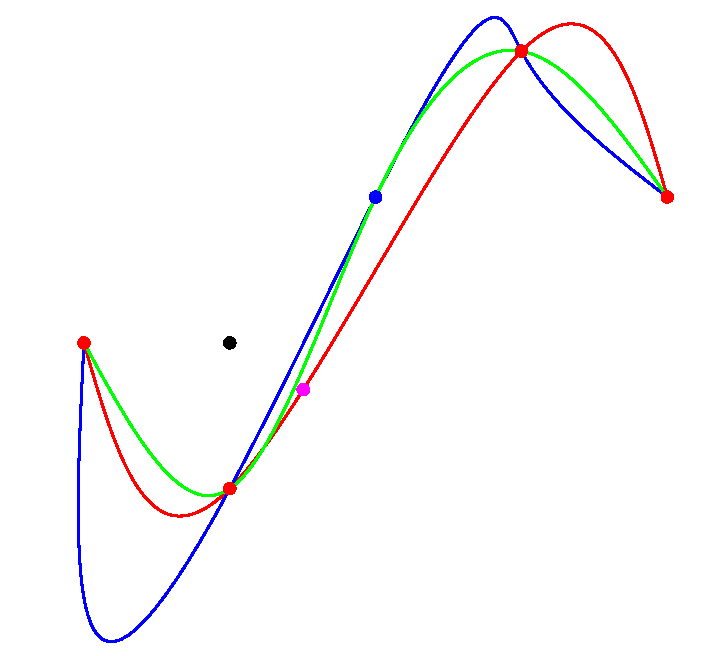
\includegraphics[width=7cm]{graficos/paramVSreparamUniform.pdf}
		  \caption{Cambio de parametrización (Uniforme)}
		  \label{fig:paramChangeUniform}
	\end{figure}
	
	\VSP
	
	\begin{figure}[H]
		  \centering
			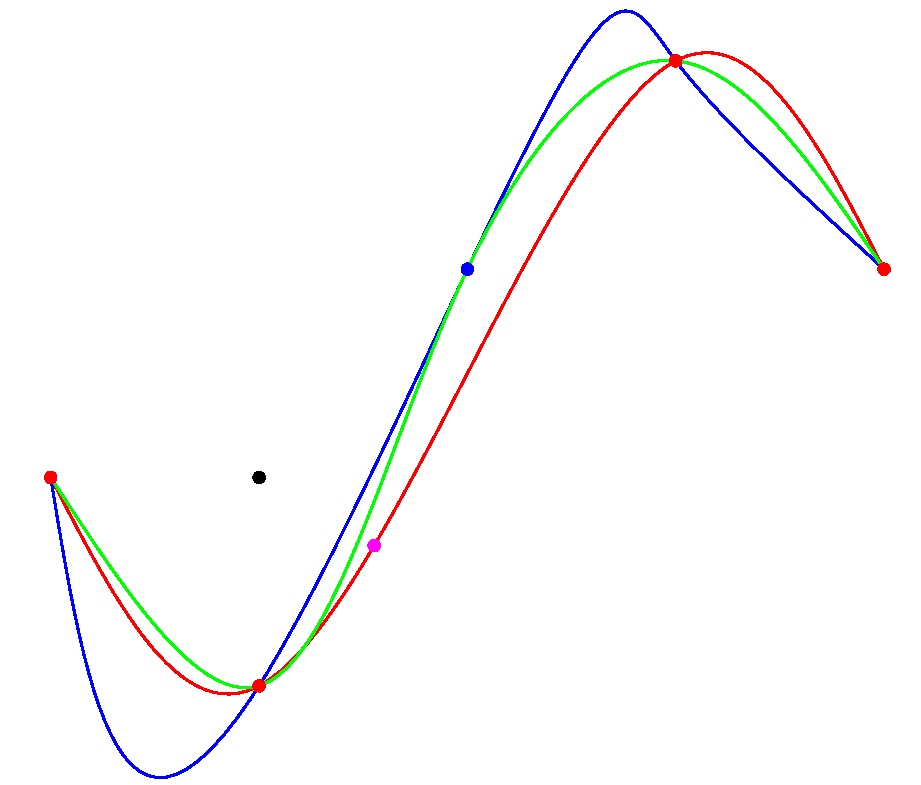
\includegraphics[width=7cm]{graficos/paramVSreparamCentripetal.pdf}
		  \caption{Cambio de parametrización (Centrípeta)}
		  \label{fig:paramChangeCentripetal}
	\end{figure}
	
	\VSP
	
	\begin{figure}[H]
		  \centering
			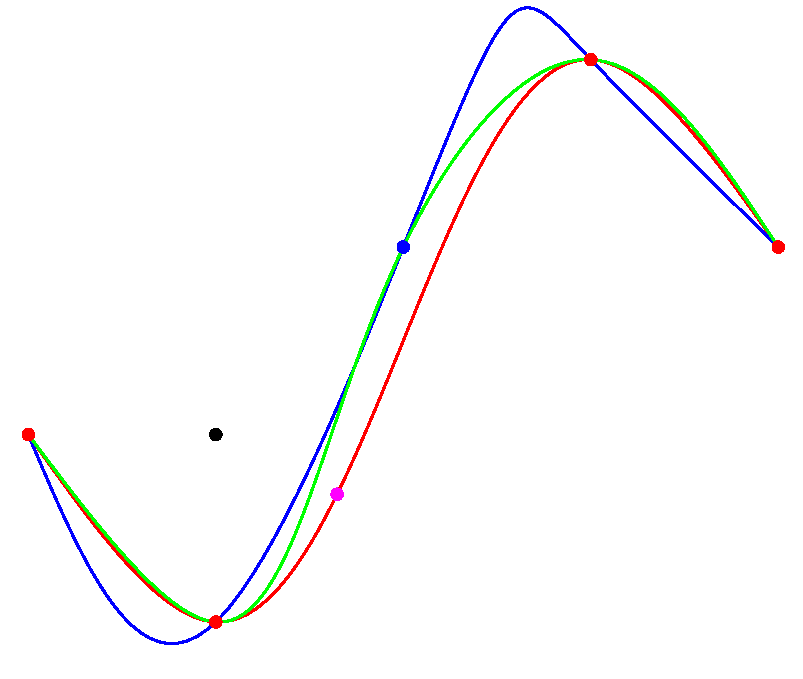
\includegraphics[width=7cm]{graficos/paramVSreparamChord.pdf}
		  \caption{Cambio de parametrización (Longitud de cuerda)}
		  \label{fig:paramChangeCHLength}
	\end{figure}
	
	\VSP
	
	Efectivamente la forma de la curva cambia al recalcular la parametrización respecto a no hacerlo. 
	
	Las curvas donde se recalcula la parametrización (curva $verde$) en las $tres$ figuras (usando cualquiera de las parametrizaciones) tienen una forma más similar a la curva original en los puntos alejados 
	al punto movido en contraste con la curva que mantiene la parametrización (curva $azul$). 
	%ya que esta cambia de manera proporcional a la distancia entre la posición del punto más próximo al elegido ($rosa$) y la posición final del mismo ($azul$).

	\end{itemize}	
\end{section}

	\newpage
	\begin{section}{Conclusiones}

\end{section}

	\newpage
	\begin{section}{Modo de compilación y uso}

\end{section}

	\newpage
	\begin{section}{Apéndices}
	\begin{subsection}{Apéndice A: Enunciado}
		\parindent = 0 pt
\parskip = 11 pt
%\usepackage[width=15.3cm, left=3.5cm, top=2.5cm, height= 24.5cm]{geometry}

\pagestyle{empty}

\newcommand{\real}{\ensuremath{\mathbb{R}}}

%\begin{document}

\begin{centering}
\bf Laboratorio de M\'etodos Num\'ericos - Primer cuatrimestre de 2011 \\
Trabajo Pr\'actico N\'umero 3: CAD - M\'as que splines \\
\end{centering}

\vskip 25pt
\hrule
\vskip 11pt

% {\bf Enunciado}

Los programas de dise\~no asistido por computadora (CAD) son herramientas fundamentales para ingenieros, arquitectos, dise\~nadores, artistas y animadores. Sus interfaces gr\'aficas esconden un sinn\'umero de complicadas operaciones. Un ejemplo b\'asico de tales operaciones es la tarea de seleccionar un punto cualquiera de una curva y moverlo a una nueva posici\'on deformando la curva. El punto seleccionado se ingresa usualmente mediante un dispositivo apuntador (\emph{mouse} o tableta digitalizadora) interactuando con la interfaz, y en general el punto ingresado est\'a meramente \emph{cerca} de la curva.

En este trabajo pr\'actico se deber\'an dise\~nar algoritmos e implementar un programa que, dadas las coordenadas $(\bar{x}_i,\bar{y}_i) \in \real^2$ de una serie de puntos de control ($i = 1..n$), construya una spline natural\footnote{Esto es suficiente para nuestro TP, pero en realidad los sistemas de CAD utilizan m\'as frecuentemente otros mecanismos para obtener, describir y manipular curvas y superficies.} param\'etrica que pase por los puntos en el orden dado. Adem\'as, dadas las coordenadas $(x^*,y^*) \in \real^2$ de un punto cercano a la curva, calcule el punto de la curva m\'as pr\'oximo y construya una nueva spline natural resultante de modificar la spline original de forma que ahora adem\'as pase por la nueva posici\'on $(\bar{x}^*,\bar{y}^*) \in \real^2$ del punto seleccionado. 
El procedimiento descripto se muestra en la figura con la spline original dibujada en l\'inea de trazos y la spline deformada en l\'inea continua.
%\begin{center}
 %\includegraphics[height=0.35\textheight]{./figura2.png}
%\end{center}

El programa deber\'a trabajar las splines como curvas param\'etricas en $\real^2$. Dadas las coordenadas de los puntos de control existen varias estrategias para definir la parametrizaci\'on. Algunas de las parametrizaciones com\'unmente utilizadas son:
\vspace{-15pt}
\begin{description}
  \setlength{\itemsep}{0pt}
  \setlength{\parskip}{0pt}
  \setlength{\parsep}{0pt}
 \item[Uniforme:] la variaci\'on del par\'ametro es igual entre cualquier par de puntos de control consecutivos;
 \item[\emph{Chord-length}:] la variaci\'on del par\'ametro entre dos puntos de control consecutivos es proporcional a la distancia entre los mismos;
 \item[Centr\'ipeta:] la variaci\'on del par\'ametro es proporcional a la ra\'iz cuadrada de la distancia entre los puntos de control\footnote{Este m\'etodo fue propuesto por Eugene Lee en \emph{Choosing nodes in parametric curve interpolation}, Computer-Aided Design 21, 1989.}.
\end{description}
\vspace{-15pt}
En este trabajo pr\'actico deber\'an utilizar alguna de estas parametrizaciones. Opcionalmente podr\'an implementar las restantes y comparar los resultados obtenidos con las tres variantes.

Adem\'as, el programa deber\'a conservar el valor del par\'ametro que le corresponde a cada punto de control y al punto seleccionado, antes y despu\'es de moverlo. 

{\bf Preguntas:}
\vspace{-15pt}
\begin{enumerate}
  \setlength{\itemsep}{0pt}
  \setlength{\parskip}{0pt}
  \setlength{\parsep}{0pt}
 \item >Depende la forma de la curva de la elecci\'on de la parametrizaci\'on? 
 \item >Cambia la forma de la curva si en lugar de deformar la curva conservando la parametrizaci\'on el programa la recalcula al mover el punto?
 \item (Opcional) >C\'omo cambia la forma de la curva seg\'un la condici\'on de borde usada (natural, sujeto, \textit{not-a-knot}, etc.)? 
 \item (Opcional) Si se quiere redibujar cont\'inuamente la curva mientras el usuario mueve el punto seleccionado, >c\'omo se puede calcular esto m\'as eficientemente?
 \item (Opcional) Luego de mover el punto seleccionado, >cambia toda la curva (\emph{control global}) o solamente una parte (\emph{control local})? >Qu\'e consecuencias puede tener esto?
 \item (Opcional) Si el intervalo del par\'ametro se muestrea uniformemente, >los puntos resultantes quedan espaciados uniformemente? >Qu\'e otras alternativas de muestreo ser\'ian apropiadas? 
 \item (Opcional) Si se necesitara que las longitudes de curva entre puntos consecutivos sean todas iguales, >c\'omo deber\'ia muestrearse?
\end{enumerate}

{\bf Archivos de entrada / salida}

La entrada de datos se realizar\'a mediante un archivo de texto con el siguiente formato:
\vspace{-15pt}
\begin{itemize}
  \setlength{\itemsep}{0pt}
  \setlength{\parskip}{0pt}
  \setlength{\parsep}{0pt}
\item En la primera l\'inea figurar\'a el n\'umero $n$ de puntos de control utilizados para definir la spline y, separado por espacio, el n\'umero $m$ de puntos de muestreo de la spline. 
\item En las siguientes $n$ l\'ineas figurar\'an las coordenadas $\bar{x}$ e $\bar{y}$ de cada punto de control separadas por espacio.
\item Una l\'inea en blanco
\item Una l\'inea con las coordenadas $x^*$ e $y^*$ del punto pr\'oximo a la curva, separadas por espacio.
\item Una l\'inea en blanco
\item Una l\'inea con las coordenadas $\bar{x}^*$ e $\bar{y}^*$ de la nueva posici\'on del punto, separadas por espacio.
\end{itemize}

La salida de datos estar\'a dada por un archivo de texto con el siguiente formato:
\vspace{-15pt}
\begin{itemize}
  \setlength{\itemsep}{0pt}
  \setlength{\parskip}{0pt}
  \setlength{\parsep}{0pt}
\item En la primera l\'inea figurar\'a el n\'umero $m$ de puntos muestreados. 
\item En las siguientes $m$ l\'ineas figurar\'an las coordenadas $x$ e $y$ de cada punto muestreado en la spline original, separadas por espacio. Estos puntos corresponder\'an a un muestreo uniforme del rango del par\'ametro e incluir\'an los extremos. De esta forma, probablemente este conjunto de puntos no incluya los puntos de control originales.
\item Una l\'inea en blanco
\item Una l\'inea con las coordenadas del punto en la curva original m\'as pr\'oximo al punto ingresado, separadas por espacio.
\item Una l\'inea en blanco
\item En las siguientes $m$ l\'ineas figurar\'an las coordenadas $x$ e $y$ de cada punto muestreado en la spline deformada, separadas por espacio.
\end{itemize}


\vskip 30pt
\hrule
\vskip 11pt

{\bf Entregas parciales}
\vspace{-15pt}
\begin{description}
  \setlength{\itemsep}{0pt}
  \setlength{\parskip}{0pt}
  \setlength{\parsep}{0pt}
 \item[10 de junio:] Implementaci\'on del c\'alculo de splines y funciones de entrada/salida.
 \item[17 de junio:] Implementaci\'on completa y verificaci\'on.
\end{description}

{\bf Entrega Final}
\vspace{-15pt}
\begin{description}
  \setlength{\itemsep}{0pt}
  \setlength{\parskip}{0pt}
  \setlength{\parsep}{0pt}
 \item[Formato Electr\'onico:] 23 de junio de 2011, hasta las 23:59 hs, a la direcci\'on: 

  {\emph{metnum.lab2011@gmail.com}}
 \item[Formato f\'isico:] 24 de junio de 2011, de 17 a 21 hs.
\end{description}

%\end{document}


	\end{subsection}
	\begin{subsection}{Apéndice B: Código fuente}
		\begin{subsection}{Modo de compilación}
			Para compilar se hace uso de la herramienta Makefile.
			
			Abrir una terminal dentro la carpeta $code$ entregada y escribir el comando "make", pulsar enter.
		\end{subsection}	
		\begin{subsection}{Modo de uso}
			Una vez compilado escriba en la terminal (posicinado sobre la misma ruta en la que lo compiló)
		\end{subsection}	
	\end{subsection}	
\end{section}

	\newpage
	\begin{section}{Referencias}

\end{section}

\end{document}
